\documentclass[9pt,aspectratio=169,xcolor=table]{beamer}

%~~~~~~~~~~~~~~~~~~~~~~~~~~~~~~~~~~~~~~~~~~~~~~~~~~~~~~~~~~~~~~~~~~~~~~~~~~~~~~
% Use roboto Font (recommended)
\usepackage[sfdefault]{roboto}
\usepackage[utf8]{inputenc}
\usepackage[T1]{fontenc}
%~~~~~~~~~~~~~~~~~~~~~~~~~~~~~~~~~~~~~~~~~~~~~~~~~~~~~~~~~~~~~~~~~~~~~~~~~~~~~~

%~~~~~~~~~~~~~~~~~~~~~~~~~~~~~~~~~~~~~~~~~~~~~~~~~~~~~~~~~~~~~~~~~~~~~~~~~~~~~~
% Define where theme files are located. ('/styles')
\usepackage{styles/fluxmacros}
\usefolder{styles}
% Use Flux theme v0.1 beta
% Available style: asphalt, blue, red, green, gray
\usetheme[style=gray]{flux}
%~~~~~~~~~~~~~~~~~~~~~~~~~~~~~~~~~~~~~~~~~~~~~~~~~~~~~~~~~~~~~~~~~~~~~~~~~~~~~~

%~~~~~~~~~~~~~~~~~~~~~~~~~~~~~~~~~~~~~~~~~~~~~~~~~~~~~~~~~~~~~~~~~~~~~~~~~~~~~~
% Extra packages
\usepackage{booktabs}
\usepackage{colortbl}
\usepackage{ragged2e}
\usepackage{amssymb}
\usepackage{multirow}
\usepackage{tikz}
\usetikzlibrary{arrows.meta, positioning, fit, backgrounds, calc, decorations.pathreplacing}
\setbeamertemplate{itemize items}[square]
\usepackage[scaled=.8]{beramono}
\usepackage{listings}
\usepackage{styles/lstlangarm}
\usepackage{array}
\definecolor{bgcolor}{HTML}{F2E9E9}
% lstlangarm.sty references \color{mauve} for string literals but never defines
% it -- only fires when a listing contains a string. Define it here.
\definecolor{mauve}{rgb}{0.58,0,0.82}
% lstlangarm's C style sets commentstyle=green!20, which is unreadable on the
% pink listing background. Darken it globally.
\lstset{commentstyle=\color{green!45!black}}
% ragged-right fixed-width column -- must be defined in the preamble, never
% inside a frame (\newcolumntype's #1 breaks beamer's frame scanner)
\newcolumntype{R}[1]{>{\RaggedRight\arraybackslash}p{#1}}
%~~~~~~~~~~~~~~~~~~~~~~~~~~~~~~~~~~~~~~~~~~~~~~~~~~~~~~~~~~~~~~~~~~~~~~~~~~~~~~
% Table striping: odd rows white, even rows very light gray.
% Needs \documentclass[...,xcolor=table]{beamer} (beamer loads xcolor itself,
% so the option must go on the class, not \usepackage).
\definecolor{stripe}{gray}{0.94}
% \striped makes body rows alternate white, gray, white, ... starting white.
% \rowcolors counts from the first coloured body row; the header is not counted.
\newcommand{\striped}{\rowcolors{1}{white}{stripe}}
%~~~~~~~~~~~~~~~~~~~~~~~~~~~~~~~~~~~~~~~~~~~~~~~~~~~~~~~~~~~~~~~~~~~~~~~~~~~~~~

%~~~~~~~~~~~~~~~~~~~~~~~~~~~~~~~~~~~~~~~~~~~~~~~~~~~~~~~~~~~~~~~~~~~~~~~~~~~~~~
% TikZ block styles -- matches ch1/ch2
% Colour variables are named identically in the book's stm32primer.tex, so any
% tikzpicture using only the \tikzset{...} styles below can be copied verbatim
% between slides and book. Only the \definecolor/\colorlet VALUES differ: the
% book is printed, so it keeps every stroke pure black with muted fills. These
% slides are projected, so both fill AND stroke are bright and saturated to
% grab attention -- see stm32primer.tex for the print palette.
\definecolor{blkfill}{HTML}{DCEBFF}
\definecolor{blkline}{HTML}{1565C0}
\definecolor{accentfill}{HTML}{FFE0B2}
\definecolor{accentline}{HTML}{E65100}
\definecolor{memfill}{HTML}{DFF5DA}
\definecolor{memline}{HTML}{2E7D32}
\definecolor{cellfill}{HTML}{FFFFFF}
\definecolor{cellline}{HTML}{424242}
\definecolor{bitmaskfill}{HTML}{DCEBFF}
\definecolor{bitmaskline}{HTML}{1565C0}
\definecolor{bithitfill}{HTML}{FFE0B2}
\definecolor{bithitline}{HTML}{E65100}
\tikzset{
  blk/.style   = {rectangle, rounded corners=2pt, draw=blkline, fill=blkfill,
                  thick, align=center, font=\small, minimum height=9mm, inner sep=3pt},
  cpublk/.style= {rectangle, rounded corners=2pt, draw=accentline, fill=accentfill,
                  thick, align=center, font=\small\bfseries, minimum height=9mm, inner sep=3pt},
  memblk/.style= {rectangle, rounded corners=2pt, draw=memline, fill=memfill,
                  thick, align=center, font=\small, minimum height=9mm, inner sep=3pt},
  cell/.style  = {rectangle, draw=cellline, fill=cellfill, align=center,
                  font=\small\ttfamily, minimum height=7mm, inner sep=2pt},
  lbl/.style   = {font=\scriptsize, text=Gray},
  flow/.style  = {-{Stealth[length=2mm]}, thick, draw=blkline},
  busline/.style={thick, draw=cellline},
}
% NOTE (theme quirks -- all fail SILENTLY, always page through the PDF):
%  - a second \\ inside a nested {...} group in a TikZ node breaks parsing
%  - {\small ...} wrapped around a nested itemize eats the frame title + list
%  - \usebeamercolor on a [plain] frame falls through to an unstyled default
%  - \newcolumntype inside a frame breaks beamer's frame scanner
%  - lstlisting needs \begin{frame}[fragile]
%  - a TikZ picture wider than its column silently overflows into neighbours
%~~~~~~~~~~~~~~~~~~~~~~~~~~~~~~~~~~~~~~~~~~~~~~~~~~~~~~~~~~~~~~~~~~~~~~~~~~~~~~

%%%%%%%%%%%%%%%%%%%%%%%%%%%%%%%%%%%
%% BEGIN CONDITIONAL COMPILATION %%
%%%%%%%%%%%%%%%%%%%%%%%%%%%%%%%%%%%
\newif\ifwebex
%\webextrue % uncomment to generate section separator
\ifwebex
\AtBeginSection[]{
  \begin{frame}
  \vfill
  \centering
  \begin{beamercolorbox}[sep=8pt,center,shadow=true,rounded=true]{title}
    \usebeamerfont{title}\insertsectionhead\par%
  \end{beamercolorbox}
  \vfill
  \end{frame}
}
\else
\AtBeginSection[]
{
{
    \setbeamercolor{background canvas}{bg=yellow!10}
    \begin{frame}[plain]
        \frametitle{Table of Contents}
        \tableofcontents[currentsection]
    \end{frame}
}
}
\fi
%%%%%%%%%%%%%%%%%%%%%%%%%%%%%%%%%%%
%% END CONDITIONAL COMPILATION   %%
%%%%%%%%%%%%%%%%%%%%%%%%%%%%%%%%%%%

%~~~~~~~~~~~~~~~~~~~~~~~~~~~~~~~~~~~~~~~~~~~~~~~~~~~~~~~~~~~~~~~~~~~~~~~~~~~~~~
% Information
\title{Synchronous Serial Interfaces: SPI and $I^2$C}
\subtitle{\emph{Introduction to ARM Cortex-M Microprocessors} --- Chapter 13}
\author{Mun\'{i}m Zabidi}
\institute{\color{primary}Faculty of Electrical Engineering, Universiti Teknologi Malaysia}
\date{\today}
\titlegraphic{assets/logoutmwhite.png}
%~~~~~~~~~~~~~~~~~~~~~~~~~~~~~~~~~~~~~~~~~~~~~~~~~~~~~~~~~~~~~~~~~~~~~~~~~~~~~~

\begin{document}

\titlepage

%===============================================================================
\section{Why This Matters}
%===============================================================================

\begin{frame}{Why This Chapter Matters}
    \begin{columns}[T]
    \begin{column}{.47\textwidth}
        {\normalsize UART has no clock wire, so both ends must agree on the baud rate. Adding a clock wire removes that need and the speed limit. SPI is fast and simple, but costs one pin per device. $I^2$C is slower, yet it connects dozens of devices on two wires. You will read a real sensor and turn its raw values into a physical measurement.}
    \end{column}
    \begin{column}{.51\textwidth}
        \begin{block}{After this chapter, you can:}
        {\small
        \begin{enumerate}\itemsep2pt
            \item Name the four SPI signals; explain full-duplex exchange.
            \item Choose CPOL and CPHA; calculate $f_{\text{SCK}}$.
            \item Configure an SPI master and do a register transaction.
            \item Describe the $I^2$C phases; explain open-drain and pull-ups.
            \item Configure an $I^2$C master and read a slave register.
            \item Choose between SPI and $I^2$C, and justify it.
            \item Convert a real sensor's output to engineering units.
        \end{enumerate}}
        \end{block}
    \end{column}
    \end{columns}
\end{frame}


%===============================================================================
\section{The SPI Bus}
%===============================================================================

\begin{frame}{Four Wires, Full Duplex}
    \begin{columns}[T]
    \begin{column}{.46\textwidth}
        \begin{center}
        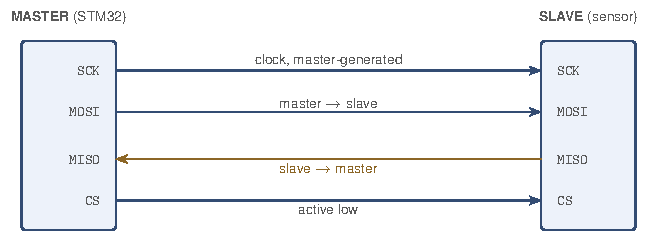
\includegraphics[width=\textwidth]{assets/spi-bus.pdf}
        \end{center}
    \end{column}
    \begin{column}{.5\textwidth}
        {\small
        \striped
        \begin{tabular}{@{}l l@{}}
            \toprule
            \textbf{Signal} & \textbf{Direction} \\
            \midrule
            \texttt{SCK}  & Master $\rightarrow$ slave \\
            \texttt{MOSI} & Master $\rightarrow$ slave \\
            \texttt{MISO} & Slave $\rightarrow$ master \\
            \texttt{CS}   & Master $\rightarrow$ slave, \alert{per device} \\
            \bottomrule
        \end{tabular}}
    \end{column}
    \end{columns}

    \vspace{3mm}
    \begin{block}{A transfer is an \emph{exchange}, not a send}
        Master and slave are one \alert{circular shift register}. Every clock edge
        shifts a bit out of each and into the other --- so sending a byte
        \emph{always} receives one at the same time. To read a device you must
        still \alert{write something} (often a dummy byte) to generate the clock.
    \end{block}
\end{frame}

\begin{frame}[plain]{Full Duplex by Shift Register}
    \begin{center}
    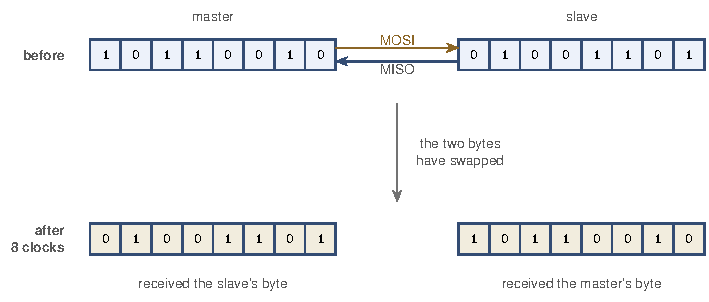
\includegraphics[width=.94\textwidth]{assets/spi-exchange.pdf}
    \end{center}

    \vspace{1mm}
    {\small\centering SPI is an \alert{exchange}, not a send or a receive. The
    two shift registers form one ring, so eight clock pulses trade their
    contents.\par}
\end{frame}

\begin{frame}[plain]{More Than One Slave}
    \begin{center}
    \includegraphics[width=.9\textwidth, height=.62\textheight, keepaspectratio]%
        {assets/spi-multi.pdf}
    \end{center}

    \vspace{1mm}
    {\small\centering \texttt{SCK}, \texttt{MOSI}, and \texttt{MISO} are
    \alert{shared} by every device; only chip select is \alert{private}.
    Adding a slave costs exactly one pin.\par}
\end{frame}

\begin{frame}[plain]{Clock Polarity and Phase}
    \begin{center}
    \includegraphics[width=.84\textwidth, height=.58\textheight, keepaspectratio]%
        {assets/spi-timing.pdf}
    \end{center}

    \vspace{2mm}
    {\small\centering \textbf{CPOL} sets the idle level of the clock;
    \textbf{CPHA} sets which edge samples the data. Four combinations, called
    \alert{modes 0 to 3} --- and the datasheet tells you which one your device
    needs.\par}
\end{frame}

\begin{frame}{Configuring an SPI Master}
    \begin{columns}[T]
    \begin{column}{.5\textwidth}
        {\ttfamily\scriptsize
        RCC->APB1ENR |= (1U << 14);~// SPI2 \\[1mm]
        SPI2->CR1 = (1U << 2)~~~~~~~// MSTR \\
        ~~~~~~~~~~| (3U << 3)~~~~~~~// BR: /16 \\
        ~~~~~~~~~~| (1U << 9)~~~~~~~// SSM \\
        ~~~~~~~~~~| (1U << 8);~~~~~~// SSI \\
        SPI2->CR1 |= (1U << 6);~~~~~// SPE}
    \end{column}
    \begin{column}{.46\textwidth}
        \begin{center}
        \fbox{\parbox{.9\textwidth}{\centering\vspace{1mm}
        $f_{\text{SCK}} = \dfrac{f_{\text{PCLK}}}{2^{(\text{BR}+1)}}$
        \vspace{1mm}}}
        \end{center}

        \vspace{2mm}
        {\small With \texttt{BR} $=3$ and a 16\,MHz peripheral clock,
        $f_{\text{SCK}} = 1$\,MHz.}
    \end{column}
    \end{columns}

    \vspace{3mm}
    \begin{block}{Why this course uses SPI2, not SPI1}
        SPI1's default \texttt{SCK} is \alert{\texttt{PA5}} --- the user LED. Using
        SPI1 would silently break every blink program in the book.

        \vspace{1mm}
        SPI2 sits on \textbf{APB1} (not APB2), and its pins \texttt{PB13}--%
        \texttt{PB15} live in \texttt{AFR[1]}, indexed as $(pin-8) \times 4$.
    \end{block}
\end{frame}

\begin{frame}[fragile]{A Register Transaction}
\begin{lstlisting}[language=C, basicstyle=\ttfamily\scriptsize]
uint8_t spi_transfer(uint8_t out)
{
    while (!(SPI2->SR & (1U << 1))) ;    // TXE -- ready to send
    *(volatile uint8_t *)&SPI2->DR = out;
    while (!(SPI2->SR & (1U << 0))) ;    // RXNE -- a byte came back
    return *(volatile uint8_t *)&SPI2->DR;
}

uint8_t read_register(uint8_t addr)
{
    cs_low();
    spi_transfer(addr | 0x80);       // bit 7 set = read
    uint8_t v = spi_transfer(0x00);  // dummy byte to clock the reply out
    cs_high();
    return v;
}
\end{lstlisting}

    \vspace{1mm}
    {\small The \alert{dummy byte} is the point: you cannot receive without
    transmitting, because the master supplies the clock.}
\end{frame}

\begin{frame}[plain]{The Complete Measurement Chain}
    \begin{center}
    \includegraphics[width=.92\textwidth, height=.68\textheight, keepaspectratio]%
        {assets/measurement-chain.pdf}
    \end{center}

    \vspace{1mm}
    {\small\centering From a physical acceleration to a number on a screen.
    Every stage is a topic from an \alert{earlier chapter}.\par}
\end{frame}

%===============================================================================
\section{I\textsuperscript{2}C}
%===============================================================================

\begin{frame}{Two Wires, Many Devices}
    \begin{columns}[T]
    \begin{column}{.5\textwidth}
        \begin{itemize}
            \item \texttt{SCL} clock and \texttt{SDA} data --- \alert{two} wires
                  total, regardless of device count
            \item Each device has a \alert{7-bit address}, so no chip-select lines
            \item Both lines are \alert{open-drain}, with external pull-ups
        \end{itemize}
    \end{column}
    \begin{column}{.46\textwidth}
        \begin{block}{Why open-drain is mandatory}
            Many devices share both wires. If two drove push-pull outputs in
            opposite directions the result would be a \alert{short circuit}.

            \vspace{2mm}
            Open-drain means a device can only \emph{pull low} or \emph{release}
            --- so the pull-up defines the idle state and no contention is
            possible.
        \end{block}
    \end{column}
    \end{columns}

    \vspace{3mm}
    {\small That is Chapter 8's open-drain output, now with a reason. The pull-up
    value follows from \alert{bus capacitance}: too large and the rising edge is
    too slow; too small and it wastes current.}
\end{frame}

\begin{frame}{A Transaction}
    \begin{center}
    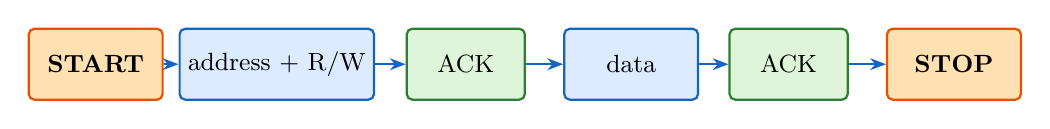
\begin{tikzpicture}[x=10mm, y=9mm]
        \node[cpublk, minimum width=17mm] (s) at (0,0)   {START};
        \node[blk,    minimum width=21mm] (a) at (2.3,0) {address $+$ R/W};
        \node[memblk, minimum width=15mm] (k) at (4.7,0) {ACK};
        \node[blk,    minimum width=17mm] (d) at (6.8,0) {data};
        \node[memblk, minimum width=15mm] (k2)at (8.8,0) {ACK};
        \node[cpublk, minimum width=17mm] (p) at (10.9,0){STOP};
        \foreach \x/\y in {s/a, a/k, k/d, d/k2, k2/p}{\draw[flow] (\x) -- (\y);}
    \end{tikzpicture}
    \end{center}

    \vspace{4mm}
    \begin{center}
    {\small
    \striped
    \begin{tabular}{@{}l R{.62\textwidth}@{}}
        \toprule
        \textbf{Phase} & \textbf{What happens} \\
        \midrule
        \textbf{START} & \texttt{SDA} falls while \texttt{SCL} is high --- the one
                         pattern that is otherwise illegal \\
        \textbf{Address} & 7 bits plus a read/write bit. Every device compares it
                           against its own \\
        \textbf{ACK} & The addressed device pulls \texttt{SDA} low. \alert{Silence
                       means nobody answered} \\
        \textbf{STOP} & \texttt{SDA} rises while \texttt{SCL} is high \\
        \bottomrule
    \end{tabular}}
    \end{center}

    \vspace{2mm}
    {\small A missing ACK is the most common I\textsuperscript{2}C fault --- and it
    usually means a \alert{wrong address} or \alert{missing pull-ups}.}
\end{frame}

\begin{frame}[plain]{The Framing Conditions, on the Wire}
    \begin{center}
    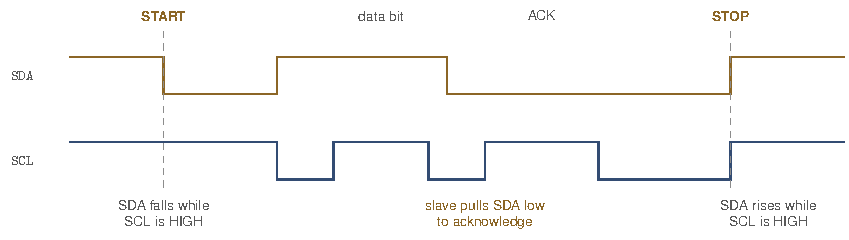
\includegraphics[width=.92\textwidth]{assets/i2c-framing.pdf}
    \end{center}

    \vspace{1mm}
    {\small\centering \texttt{SDA} may only change while \texttt{SCL} is LOW,
    so the two transitions that occur while \texttt{SCL} is HIGH are
    \alert{unambiguous markers} for the start and end of a transfer.\par}
\end{frame}

\begin{frame}[plain]{Many Devices on Two Wires}
    \begin{center}
    \includegraphics[width=.86\textwidth, height=.6\textheight, keepaspectratio]%
        {assets/i2c-multi.pdf}
    \end{center}

    \vspace{1mm}
    {\small\centering Compare this with SPI's three private chip-select
    lines: here the pin count stays at \alert{two}, no matter how many
    devices hang off the bus --- selection has moved into \alert{software}.\par}
\end{frame}

\begin{frame}{Choosing Between Them}
    \begin{center}
    {\small
    \striped
    \begin{tabular}{@{}l l l@{}}
        \toprule
         & \textbf{SPI} & \textbf{I\textsuperscript{2}C} \\
        \midrule
        Wires & 4, plus one CS \alert{per device} & \alert{2}, regardless of count \\
        Speed & \alert{Tens of MHz} & 100\,kHz to 1\,MHz \\
        Duplex & Full & Half \\
        Addressing & A chip-select line & A \alert{7-bit address} \\
        Acknowledge & None --- you cannot tell if it worked & \alert{ACK} per byte \\
        Best for & Displays, flash, fast ADCs & Many slow sensors, EEPROM \\
        \bottomrule
    \end{tabular}}
    \end{center}

    \vspace{3mm}
    \begin{block}{The trade in one sentence}
        \alert{SPI buys speed with pins}; \alert{I\textsuperscript{2}C buys pins
        with speed} --- and throws in an acknowledgement, so you know whether the
        device is actually there.
    \end{block}
\end{frame}

\begin{frame}{An SPI Byte at Five Levels}
    \begin{center}
    {\small
    \striped
    \begin{tabular}{@{}l R{.65\textwidth}@{}}
        \toprule
        \textbf{Level} & \textbf{Representation} \\
        \midrule
        Physical    & Eight clock pulses on PB13; data levels on PB15 and PB14 \\
        Hardware    & Two shift registers exchanging contents in a ring \\
        Register    & \texttt{SPI2->DR} written, then read \\
        C           & \texttt{value = spi\_transfer(0x00);} \\
        Engineering & One axis of acceleration, in units of g \\
        \bottomrule
    \end{tabular}}
    \end{center}

    \vspace{3mm}
    \begin{block}{You have now met every peripheral this book teaches}
        Digital pins, interrupts, timers, analog input, and three serial
        buses: one asynchronous and two synchronous. Chapter~14 asks you
        to use them \alert{all at once}, with no OS to arbitrate.
    \end{block}
\end{frame}

\begin{frame}{Summary}
	\begin{columns}[c]
		\begin{column}{.62\textwidth}
			\begin{center}
				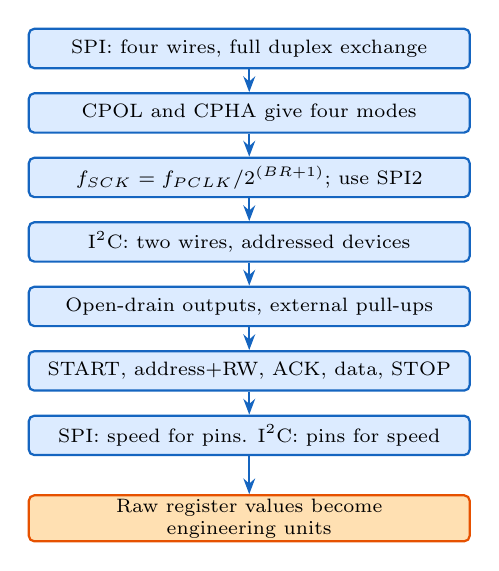
\begin{tikzpicture}[x=10mm, y=7.8mm]
					\node[blk, minimum width=56mm, minimum height=5.0mm, inner sep=1.2pt, font=\scriptsize] (n0) at (0,0.00) {SPI: four wires, full duplex exchange};
					\node[blk, minimum width=56mm, minimum height=5.0mm, inner sep=1.2pt, font=\scriptsize] (n1) at (0,-1.05) {CPOL and CPHA give four modes};
					\node[blk, minimum width=56mm, minimum height=5.0mm, inner sep=1.2pt, font=\scriptsize] (n2) at (0,-2.10) {$f_{\text{SCK}} = f_{\text{PCLK}}/2^{(\text{BR}+1)}$; use SPI2};
					\node[blk, minimum width=56mm, minimum height=5.0mm, inner sep=1.2pt, font=\scriptsize] (n3) at (0,-3.15) {I\textsuperscript{2}C: two wires, addressed devices};
					\node[blk, minimum width=56mm, minimum height=5.0mm, inner sep=1.2pt, font=\scriptsize] (n4) at (0,-4.20) {Open-drain outputs, external pull-ups};
					\node[blk, minimum width=56mm, minimum height=5.0mm, inner sep=1.2pt, font=\scriptsize] (n5) at (0,-5.25) {START, address+RW, ACK, data, STOP};
					\node[blk, minimum width=56mm, minimum height=5.0mm, inner sep=1.2pt, font=\scriptsize] (n6) at (0,-6.30) {SPI: speed for pins. I\textsuperscript{2}C: pins for speed};
					\node[cpublk, minimum width=56mm, minimum height=5.0mm, inner sep=1.2pt, font=\scriptsize, align=center] (n7) at (0,-7.65) {Raw register values become\\engineering units};
					\foreach \a/\b in {0/1,1/2,2/3,3/4,4/5,5/6,6/7}{\draw[flow] (n\a) -- (n\b);}
				\end{tikzpicture}
			\end{center}
		\end{column}
		\begin{column}{.34\textwidth}
			{\scriptsize
				\textbf{Terminology covered}\\[1mm]
				\begin{itemize}
					\item MOSI, MISO, SCK, CS
					\item CPOL, CPHA
					\item Open-drain, pull-up
					\item START, ACK, STOP
				\end{itemize}
				\vspace{3mm}
				\textbf{Next: Chapter 14}\\[1mm]
				\emph{Designing, Building and Verifying}\\[1mm]
				Every peripheral so far, in one program, at once.}
		\end{column}
	\end{columns}
\end{frame}

\end{document}

